\RequirePackage{plautopatch}
\RequirePackage[l2tabu, orthodox]{nag}

\documentclass[dvipdfmx]{jlreq}
\usepackage{graphicx}
\usepackage{natbib}
\usepackage{hyperref}
\usepackage{amsmath}
\usepackage{amssymb}
\usepackage{float}

\title{
\vspace{-4cm}
モデルの修正（金融仲介業者の導入）
}

\author{
  岸本康佑
  \thanks{
  Email: \texttt{s12102301404@toyo.jp}, \texttt{kishimoto.research@gmail.com} \\
  GitHub: \url{https://github.com/Kishimoto-econ}
}}
\date{2026年7月6日}

\begin{document}
\maketitle

%本文開始
\section{主な変更点}
\begin{itemize}
  \item Kiyotaki and Moore (1997)にGertler and Karadi (2011)の金融仲介業者（Financial intermediaries）を導入
  \item FarmerとGathererの利子率を区別
  \item Gatherの予算制約式に，金融仲介業者からの資産移転を追加（モデル構築の技術的に必要）
  \item この変更により，変数$\chi_t, \nu_t, \eta_t, \zeta_t, N_t, \phi_t, N_{et}, N_{nt}$と，パラメータ$\beta^{FI}, \theta, \rho, \omega$が増加
\end{itemize}

\section{Farmer}
\begin{align}
  \max_{x_t, b_t, k_t} \quad & \mathbb{E}_t \bigg( \sum_{s=0}^{\infty} \beta^s x_{t+s} \bigg) \label{eq:f_u} \\
  \text{s.t.} \quad & q_t(k_t - k_{t-1}) + R_t b_{t-1} + x_t - c k_{t-1} = a k_{t-1} + b_t \label{eq:f_yosan} \\
  & R_t b_t \leq q_{t+1} k_t \label{eq:kariire}\\
  & x_t \geq c k_{t-1} \label{eq:syouhi}
\end{align}
\begin{itemize}
  \item $R$を$R_t$に変更
\end{itemize}
自家消費制約のオイラー方程式は，
\begin{equation}
  1 + \varphi_t = (\beta(1+\varphi_{t+1}) + \mu_t) R_t
\end{equation}
に変更．

\section{Gatherer}
\begin{align}
  \max_{x^\prime_t, b^\prime_t, k^\prime_t, q_t} \quad & \mathbb{E}_t \bigg( \sum_{s=0}^{\infty} (\beta^\prime)^s x^\prime_{t+s} \bigg) \label{eq:g_u} \\
  \text{s.t.} \quad & q_t(k^\prime_t - k^\prime_{t-1}) + R^\prime_t b^\prime_{t-1} + x^\prime_t = (z+k^\prime)^\alpha + \Pi^\prime_t + b^\prime_t \label{eq:g_yosan} \\
  \text{where} \quad & \Pi^\prime_t = (1-\theta-\omega) b_{t-1}
\end{align}
\begin{itemize}
  \item 予算制約式に金融仲介業者からの資産移転$\Pi_t$を追加（モデル構築の技術的に必要）
  \item $\omega$は資産移転の額に関するパラメータ，$\theta$は金融仲介業者が存続する割合（詳しくはGertler and Karadi (2011)の研究ノートを参照）
\end{itemize}
オイラー方程式の変更はなし．

\section{金融仲介業者}
以下，Gertler and Karadi (2011)の研究ノートの数式を本研究の表現に書き換える．リストの式番号は研究ノートに対応している．
\begin{itemize}
  \item (1)式
    \begin{equation}
      b_t = N_t + b^\prime_{t+1}
    \end{equation}

  \item (2)-(4)式
    \begin{equation}
      N_{t+1} = (R_{t+1} - R^\prime_{t+1}) b_t + R^\prime_{t+1} N_t
    \end{equation}

  \item (5)式
    \begin{equation}
      \mathbb{E}_t (\beta^{FI})^s (R_{t+s+1} - R^\prime_{t+s+1}) \geq 0,
      \qquad s \geq 0
    \end{equation}
    ※$\beta^{FI}$は金融仲介業者（Financial Intermediaries）の割引率．

  \item (6)-(7)式
    \begin{equation}
      V_t = \max \mathbb{E}_t \sum_{s=0}^\infty (1-\theta) \theta^s (\beta^{FI})^{s+1} [(R_{t+s+1} - R^\prime_{t+s+1}) b_{t+s} + R^\prime_{t+s+1} N_{t+s}]
    \end{equation}

  \item (8)式
    \begin{equation}
      V_t \geq \rho b_t
    \end{equation}
    ※$\lambda$はラグランジュ乗数で使っているので，$\rho$に変更．

  \item (9)-(13)式
    \begin{align}
      V_t &= \nu_t \cdot b_t + \eta_t N_t \\
      &with \\
      \nu_t &= \mathbb{E}_t \{ (1-\theta) (\beta^{FI}) (R_{t+1} - R^\prime_{t+1}) + (\beta^{FI}) \theta \chi_{t+1} \nu_{t+1} \} \\
      \eta_t &= \mathbb{E}_t \{ (1-\theta) + (\beta^{FI}) \theta \zeta_{t+1} \eta_{t+1} \} \\
      &where \\
      \chi_{t+s} &\equiv \frac{b_{t+s}}{b_t} \\
      \zeta_{t,t+s} &\equiv \frac{N_{t+s}}{N_t}
    \end{align}
    ※$z$はGathererの生産関数で使っているので，$\zeta$に変更．
  \item (14)式
    \begin{equation}
      \eta_t N_{t} + \nu_t b_t \geq \rho b_t
    \end{equation}

  \item (15)式
    \begin{equation}
      b_t = \frac{\eta_t}{\rho-\nu_t} N_{t} = \phi_t N_{t}
    \end{equation}

  \item (16)式
    \begin{equation}
      N_{t+1} = [(R_{t+1} - R^\prime_{t+1}) \phi_t + R^\prime_{t+1}] N_{jt}
    \end{equation}

  \item (17)-(18)式
    \begin{align}
      \zeta_{t+1} &= N_{t+1} / N_t = (R_{t+1} - R^\prime_{t+1}) \phi_t + R^\prime_{t+1} \\
      \chi_{t+1} &= b_{t+1} / b_t = (\phi_{t+1} / \phi_t) \zeta_{t+1}
    \end{align}

  \item (19)式
    \begin{equation}
      b_t = \phi_t N_t
    \end{equation}

  \item (20)式
    \begin{equation}
      N_t = N_{e, t} + N_{n, t}
    \end{equation}

  \item (21)式
    \begin{equation}
      N_{et} = \theta [(R_t - R^\prime_t) \phi_{t-1} + R^\prime_t] N_{t-1}
    \end{equation}

  \item (22)式
    \begin{equation}
      N_{n, t} = \omega b_{t-1}
    \end{equation}

  \item (23)式
    \begin{equation}
      N_t = \theta [(R_t - R^\prime_t) \phi_{t-1} + R^\prime_t] N_{t-1} + \omega b_{t-1}
    \end{equation}
\end{itemize}

\newpage

\section{Full model}
\subsection{Farmer}
\begin{gather}
  q_t(k_t-k_{t-1})+R_tb_{t-1}+x_t-ck_{t-1} = ak_{t-1}+b_t \\
  R_tb_t = q_{t+1}k_t \\
  x_t = ck_{t-1} \\
  1+\varphi_t = (\beta(1+\varphi_{t+1})+\mu_t)R_t \\
  q_t(1+\varphi_t)+\beta c\varphi_{t+1} = \beta(1+\varphi_{t+1})(a+c+q_{t+1})+\mu_tq_{t+1}
\end{gather}

\subsection{Gatherer}
\begin{gather}
  q_t = \beta'\left[\alpha(z+k'_t)^{\alpha-1}+q_{t+1}\right]
\end{gather}

\subsection{Financial intermediary}
\begin{gather}
  \nu_t = E_t\left[(1-\theta)\beta^{FI}\left(R_{t+1}-\frac1{\beta'}\right)+\beta^{FI}\theta\chi_{t+1}\nu_{t+1}\right] \\
  \eta_t = E_t\left[(1-\theta)+\beta^{FI}\theta\zeta_{t+1}\eta_{t+1}\right] \\
  \phi_t = \frac{\eta_t}{\rho-\nu_t} \\
  b_t = \phi_tN_t(1-\varepsilon_t) \label{eq:a} \\
  \zeta_{t+1} = (R_{t+1}-\frac{1}{\beta'})\phi_t+\frac{1}{\beta'} \\
  \chi_{t+1} = \frac{\phi_{t+1}}{\phi_t}\zeta_{t+1} \\
  N_t = N_{et}+N_{nt} \\
  N_{et} = \theta\left[(R_t-\frac{1}{\beta'})\phi_{t-1}+\frac{1}{\beta'}\right]N_{t-1} \\
  N_{nt} = \omega b_{t-1}
\end{gather}
※総量規制ショック$(1-\varepsilon_t)$を\eqref{eq:a}式に入れた．

\subsection{Market clearing}
\begin{gather}
  x_t+mx'_t+R_tb_{t-1}+\frac1{\beta'}b'_{t-1} = Y_t+m(1-\theta-\omega)b_{t-1} \\
  Y_t = (a+c)k_{t-1}+m(z+k'_t)^{\alpha} \\
  k_t+mk'_t = \bar K \\
  b_t+mb^\prime_t = 0
\end{gather}

\section{IRFの簡単な考察}
\begin{itemize}
  \item 1期目のみであるが，Farmerの借入金$b$と不動産価格$q$が総量規制ショック$(1-\varepsilon_t)$によって下落
  \item 2期目以降から戻っているのは，ショックによって減少した貸出$b_t$を増加させる（定常状態に戻す）ために，Farmerの金利$R_t$が下落しているからである（Kiyotaki-Mooreモデルはこれを防ぐために金利を固定化した）
  \item よって，$R$を内生変数ではなく一定にしなければならないが，一定にすると内生変数の数が1つ減るので，方程式を一本減らさなければならない（これが難しい）
  \item $R$の市場調整の動きを消せれば，目的のモデルが完成するかもしれない！！
  \item 加えて，公定歩合の引き上げでFarmerの金利が上昇したというショックを与えることができた場合，総量規制ショックのみではショックは1期のみだが，公定歩合の引き上げによって総量規制ショックの影響が増幅されたというモデルを作ることもできる
\end{itemize}

\begin{figure}
  \centering
  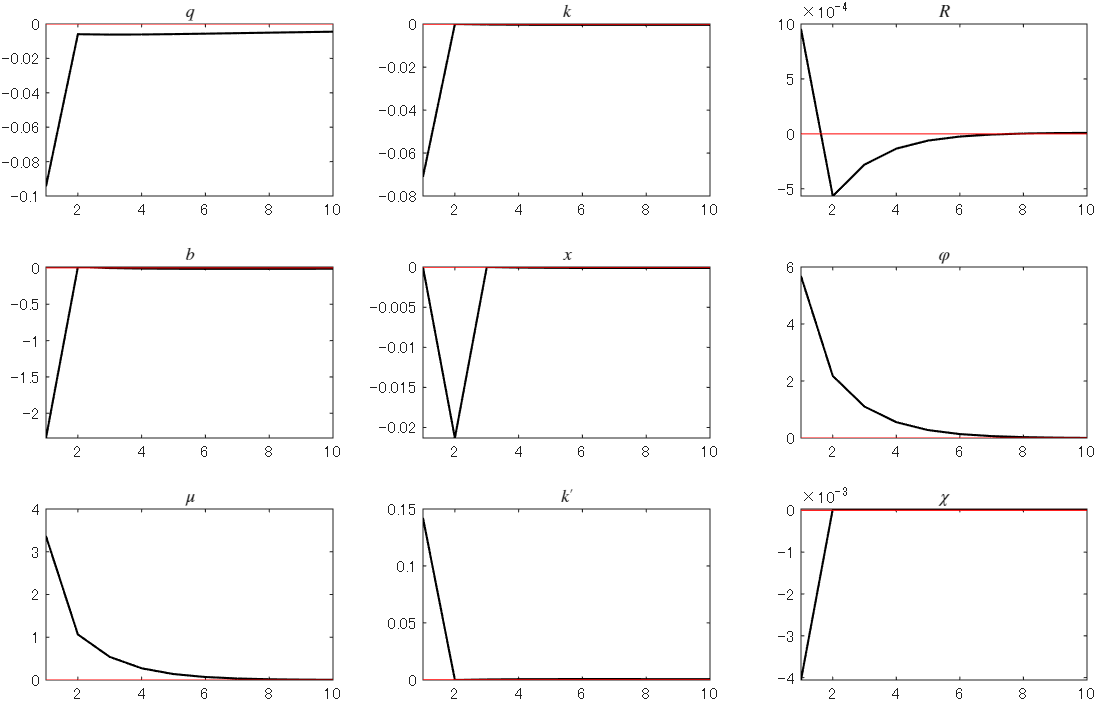
\includegraphics[scale=0.8]{fig_1.png}
\end{figure}

\begin{figure}
  \centering
  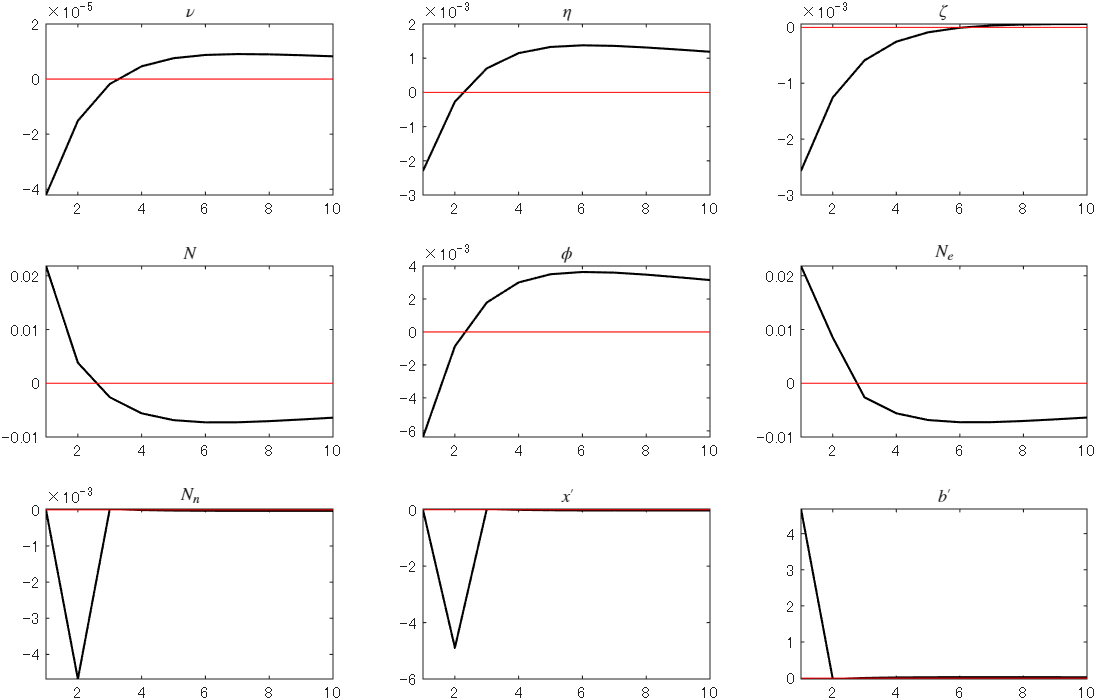
\includegraphics[scale=0.8]{fig_2.png}
\end{figure}

\begin{figure}[H]
  \centering
  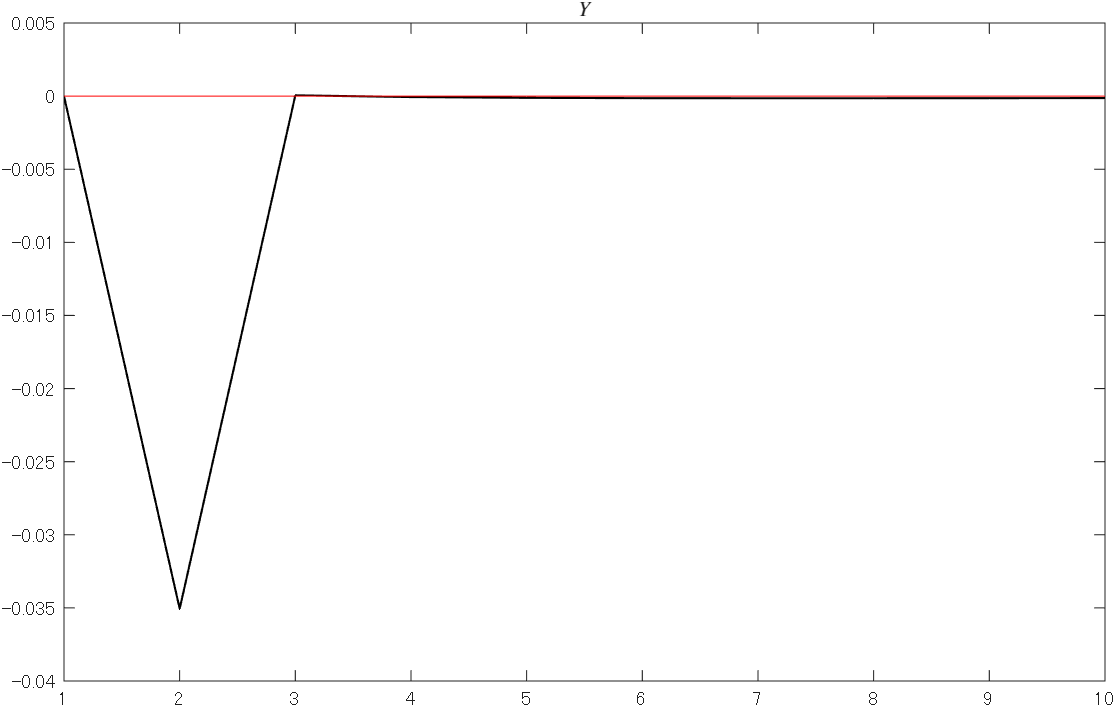
\includegraphics[scale=0.4]{fig_3.png}
\end{figure}




\end{document}







